%====================================================
% 第2章：理論
%====================================================

\section{理論}
\subsection{系統連系システム}
Fig.\ref{fig:grid}に三相NPP(Neutral Point Piloted)型3レベルインバータを用いた系統連系システムを示す．
本システムは分散型電源$Edc$から供給される直流電圧をレベルインバータで$0V,±Edc/2 V,±EdcV$
の矩形波電圧へ変換する．その後インダクタ$L_1$とコンデンサ$C$によって構成された
フィルタで平滑化され，系統リアクトル$L_t$を介して系統電圧$V_S$に接続される\cite{ref05}．

\begin{figure}[htbp]
    \centering
     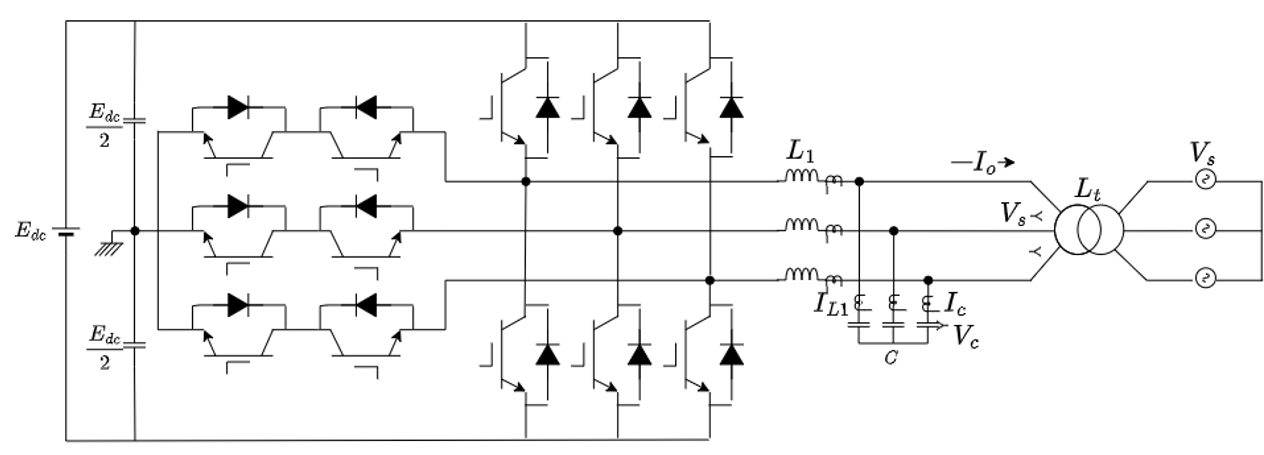
\includegraphics[width=0.5\textwidth]{figures/grid.png}
    \caption{Three-phase grid-tied inverter system}
    \label{fig:grid}
\end{figure}

Fig.\ref{fig:control.png}に制御ブロック図を示す．
本システムの制御対象はインダクタ電流$I_{L1}$とし，
インダクタ電流$I_{L1}$を指令値$I_{L1}^*$に追従させることを考える．
制御対象の各相からインダクタ電流$I_{L1}$，コンデンサ電圧$V_C$，
コンデンサ電流$I_C$を取得する．
取得した各相の状態量に対して三相二相変換を適用することで，
三相システムを独立した2つの単相システムに分離することができる．
操作量を導出し，二相三相変換を適用することでU相及びV相，W相における操作量を求める．
導出された操作量を三角波と比較することで各相のゲート信号を生成する\cite{ref06}．
\begin{figure}[htbp]
    \centering
     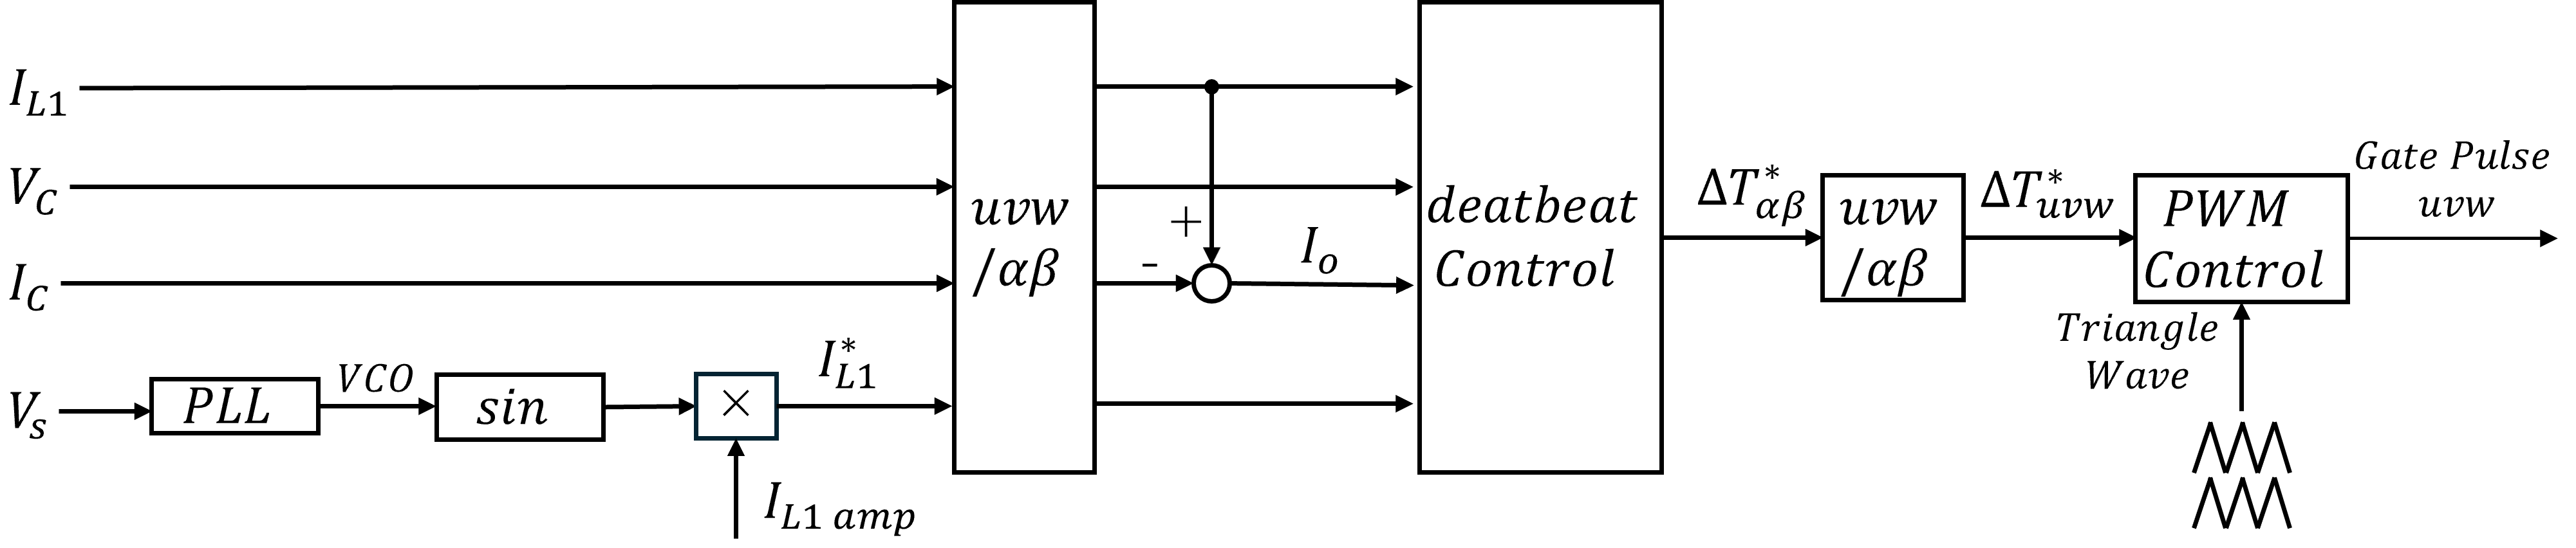
\includegraphics[width=0.5\textwidth]{figures/control.png}
    \caption{Control block diagram of Deadbeat control}
    \label{fig:control.png}
\end{figure}


\subsection{疑似dq変換を用いたPLL制御}

Fig.\ref{fig:PLL}にPLL制御のブロック図を示す．
系統電圧に三相二相変換，dq変換を適用し，位相差を算出する．
PI制御は位相差が0となるように制御し，周波数を算出する．
VCO(Voltage Controlled Oscillator)は周波数から位相を生成するためにを用いる．\\

\begin{figure}[htbp]
    \centering
     
\includegraphics[width=0.5\textwidth]{figures/PLL.png}
    \caption{Block diagram of PLL control}
    \label{fig:PLL}
\end{figure}

Fig.\ref{fig:quasi_dq}に疑似dq変換を用いたPLL制御ブロック図を示す．
対象となる系統が単相である場合，単純に直交座標系に変換できない．
疑似dq変換を用いることで単相の場合でも位相と振幅を算出することが可能である．
疑似dq変換では3サンプリング分のデータを取得し，
1サンプリング前の系統電圧を実数部，現在の系統電圧と2サンプリング前の系統電圧差分を取り，
三角関数の積差の公式を用いて虚数部を算出することで直交座標系に変換することができる．
$z$は遅れ演算子である．\\

\begin{figure}[htbp]
    \centering
     
\includegraphics[width=0.5\textwidth]{figures/quasi_dq.png}
    \caption{Block diagram of PLL control using quasi-dq transformation}
    \label{fig:quasi_dq}
\end{figure}


疑似dq変換では，サンプリング周波数を高くすることにより高速な応答が得られるが，
電圧に含まれるノイズの影響が大きくなり，精度の高い検出が難しくなる．
逆に，サンプリング周波数を低くすることでノイズの影響を低減させることができるが，
応答性は悪くなる．
これに対し，複数のサンプリング周波数を並列に演算し，その出力の平均を取ることによってノイズの影響を低減している．
先行研究では，1MHz,10kHz,6.7kHz,5kHzの4つのサンプリング周波数を用いている\cite{ref04}．
Fig.\ref{fig:dq_proposed}に10MHz，3kHzのサンプリング周波数を用いた疑似dq変換のシミュレーション結果を示す．
Fig.\ref{fig:dq_proposed}より，10MHzにおいてノイズ成分が強調されるとき，3kHzでは減衰している．
応答の異なる周波数を組み合わせることで，各サンプリングが持つノイズ成分を相互に補完し合うことが可能となる．
また，10kHz，6.7kHz，3kHzの各サンプリング点は互いにずれるため，
特定の周波数成分に含まれるノイズの重畳することを回避できる．
よって，本研究では10MHz，10kHz，6.7kHz，3kHzのサンプリング周波数を並列化する疑似dq変換を提案する．
Fig.\ref{fig:dq_costom}に本論文で提案する疑似dq変換を用いたPLL制御ブロック図を示す．

\begin{figure}[htbp]
    \centering
     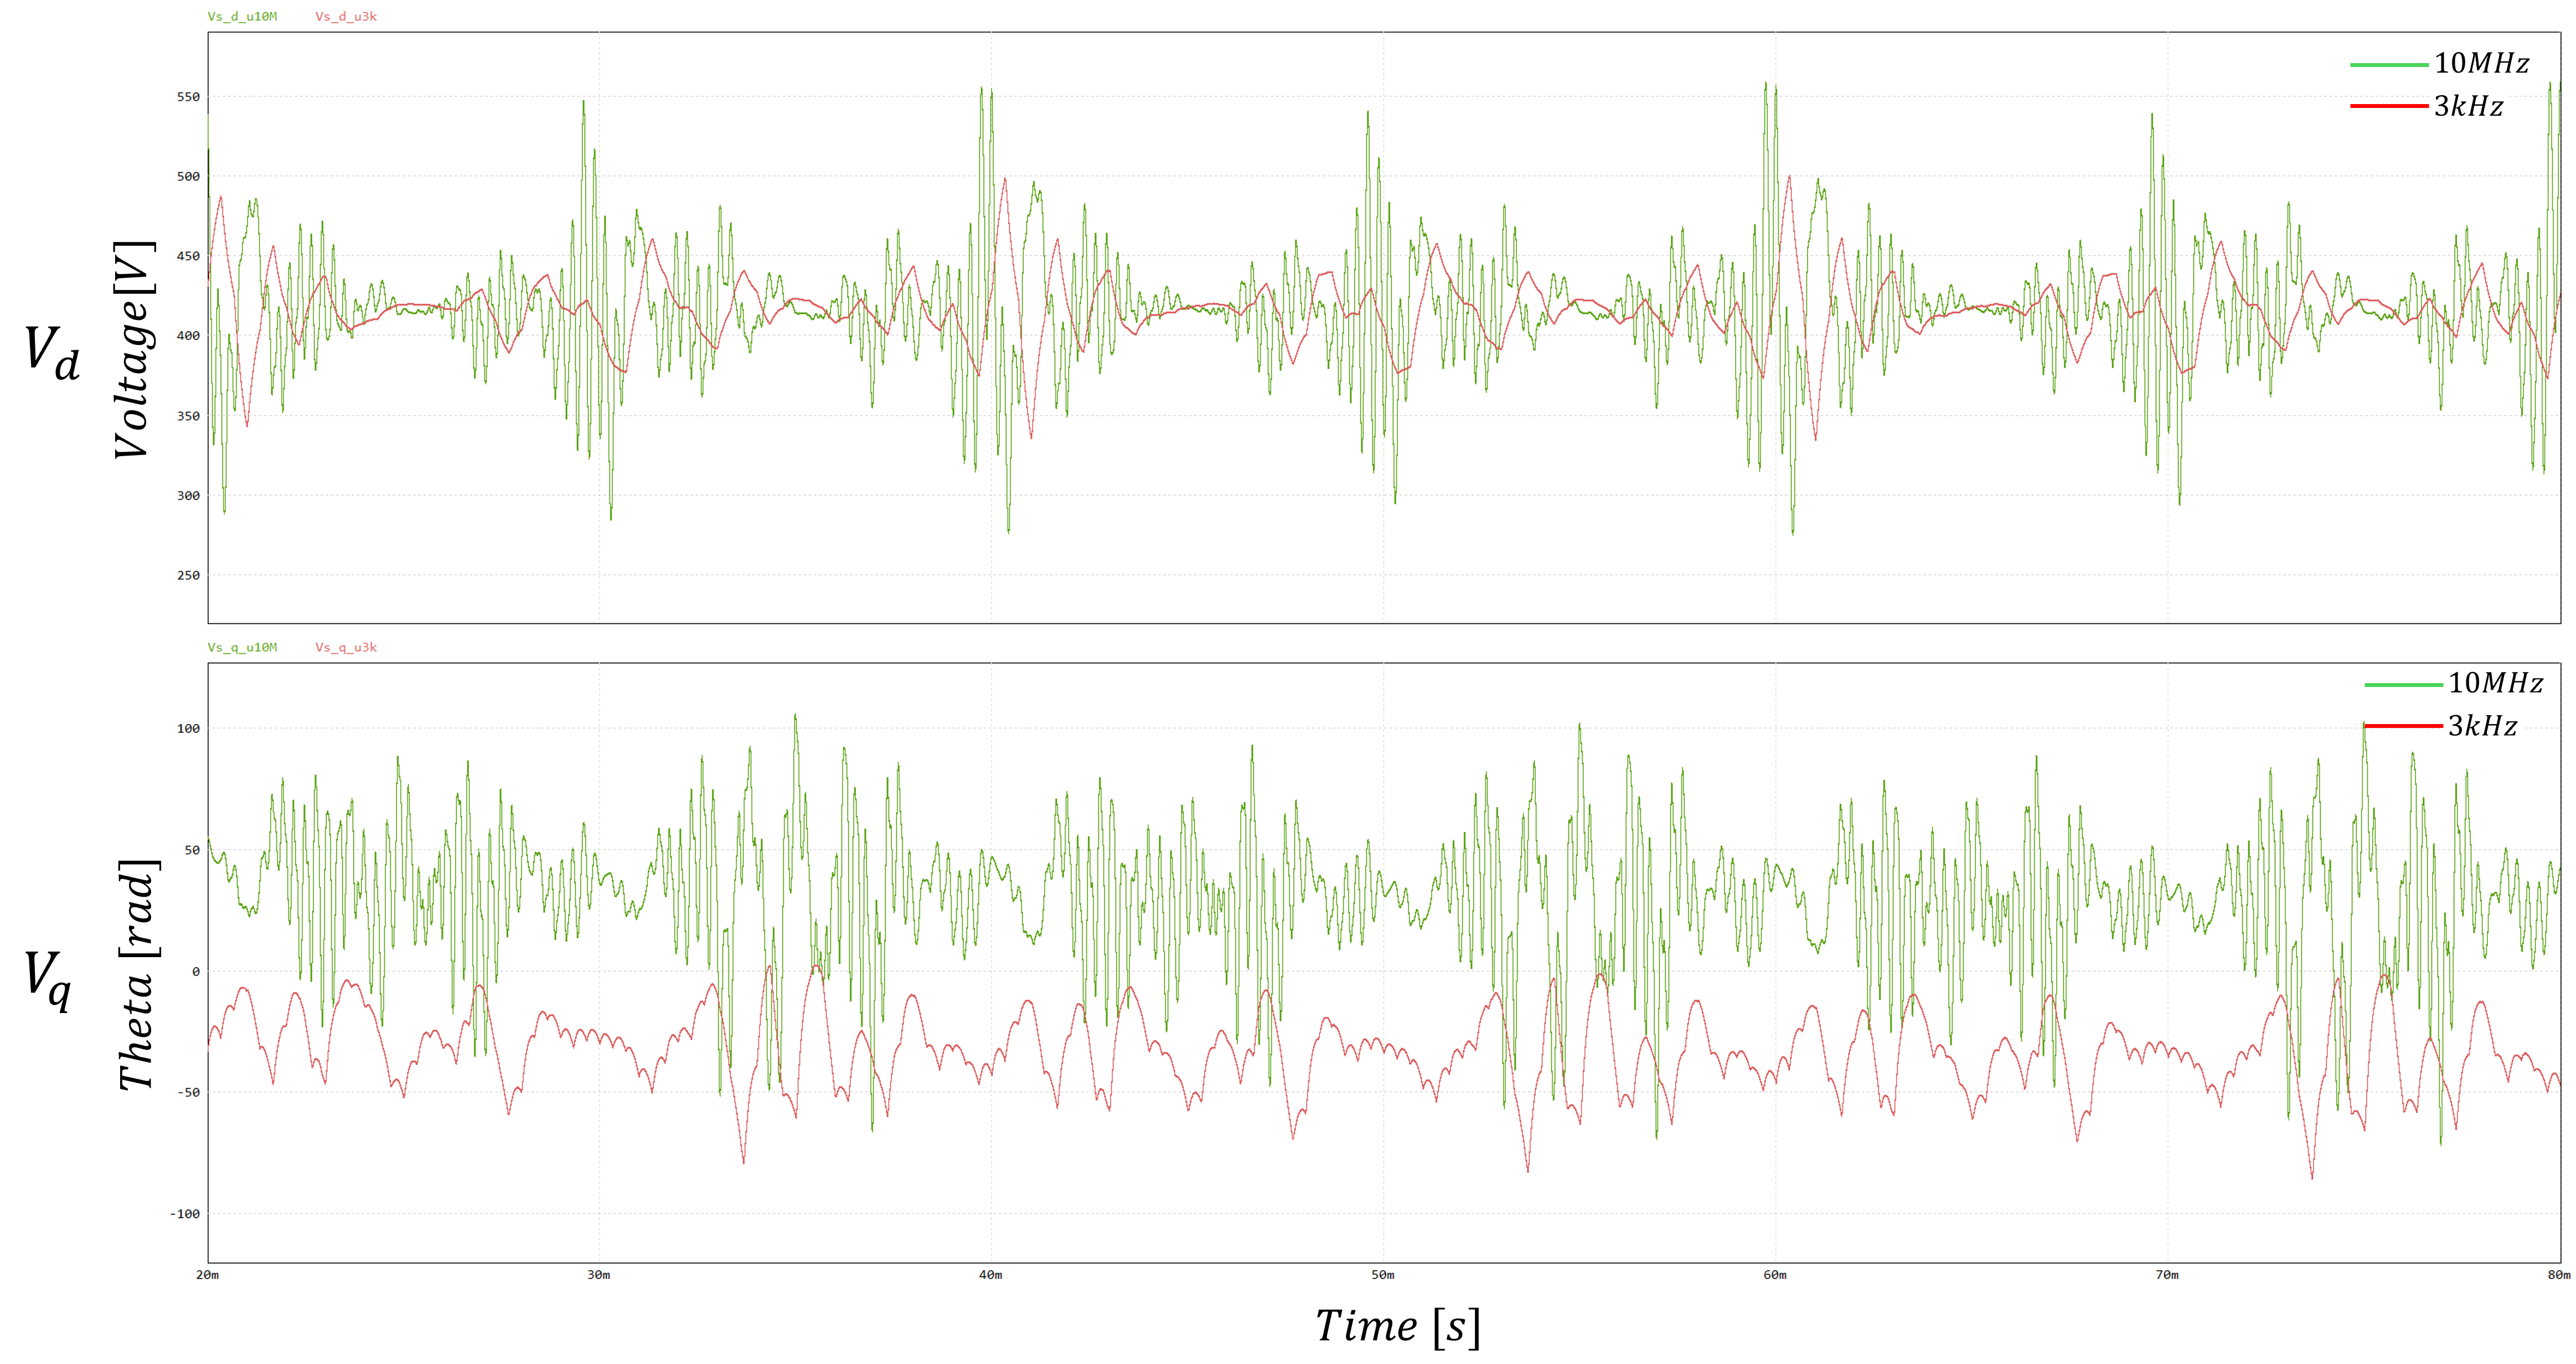
\includegraphics[width=0.5\textwidth]{figures/dq_proposed.png}
    \caption{Quasi dq transformation(10MHz,3kHz)}
    \label{fig:dq_proposed}
\end{figure}

\begin{figure}[htbp]
    \centering
     
\includegraphics[width=0.5\textwidth]{figures/dq_costom.png}
    \caption{Block diagram of proposed method}
    \label{fig:dq_costom}
\end{figure}

対象となる系統電圧を\eqref{eq:1}式のように余弦波として表されるものとする．
また，サンプリング周期を$T_s$としたときに，1サンプル時間前の系統電圧は\eqref{eq:2}式のように表される．
これを実数部$V_{re}$とする．さらに2サンプル時間前の系統電圧は\eqref{eq:3}式のように表される．
ここで，$V_{L}$は系統電圧の最大振幅値である．

\begin{equation}
V_S(k) = V_L \cos(\omega t)\label{eq:1} 
\end{equation}
\begin{equation}
V_S(k-1) = V_L \cos(\omega(t-T_s) )=V_{re}\label{eq:2} 
\end{equation}
\begin{equation}
V_S(n-2) = V_L \cos(\omega(t-2T_s))\label{eq:3} 
\end{equation}

式\eqref{eq:1}と式\eqref{eq:3}の差分を取ると，三角関数の積差の公式である式\eqref{eq:4}を用いることで式\eqref{eq:5}を得られる．

\begin{align}
\cos u - \cos v &= -2 \sin \frac{u+v}{2} \sin \frac{u-v}{2} \label{eq:4}  \\
V_s(k-2) - V_s(k) &= V_m \{ \cos(\omega(t-2T_s)) - \cos \omega t \} \notag \\
&= V_m \{ 2 \sin(\omega T_s) \sin(\omega (t-T_s)) \} \notag \\
\frac{V_s(k-2) - V_s(k)}{2\omega T_s} &= \frac{V_m}{\omega T_s} \{ \sin(\omega T_s) \sin(\omega (t-T_s)) \} \notag \\
&\fallingdotseq V_m \sin(\omega (t-T_s)) = V_{Im} \label{eq:5} 
\end{align}

式\eqref{eq:5}は式\eqref{eq:2}に比べて位相が90°遅れた波形となるため，これにdq変換を適用することで，
3サンプリング分のデータから位相と振幅を求めることが可能である\cite{ref07}．

\subsection{複素係数フィルタ}
実係数フィルタの場合，バンドパス特性を有するためには
最低でも2次のIIRフィルタとして構成しなければならないが，
複素係数フィルタの場合，1次のIIRフィルタとして構成できる．
\eqref{eq:6}式に1次の複素係数バンドパスフィルタの伝達関数，
Fig.\ref{fig:complex_diagram}にブロック線図を示す.
ここで，$r$は通過域の帯域を決めるパラメータ$(0<r<1)$，
$\Omega_d$はサンプリングレートで正規化した通過域の中心角周波数$(-\pi<Ω_d<\pi)$，
フィルタ係数$re^{j\Omega_d}$は複素数である．
また，複素係数バンドパスフィルタの状態方程式は\eqref{eq:7}式，出力方程式は\eqref{eq:8}式となる．
ただし，入力変数$u$，状態変数$x$，出力変数$y$は複素数となる．
\begin{equation}
Y(z) = \frac{1-r}{1-re^{j\Omega_d}z^{-1}}U(z)\label{eq:6} 
\end{equation}
\begin{equation}
x(k) = u(k)+1-re^{j\Omega_d}x(k-1)\label{eq:7} 
\end{equation}
\begin{equation}
y(k) = (1-r)x(k)\label{eq:8} 
\end{equation}
　
バンドパスフィルタの通過域の中心周波数 $f_o$ =50[Hz]を
サンプリング周波数 $f_s$ =10[kHz]で正規化すると，
中心角周波数$Ω_d$は\eqref{eq:9}式で得られる．

\begin{equation}
\Omega_d = 2\pi f_o/f_s \simeq 0.0314 \label{eq:9} 
\end{equation}
　

\begin{figure}[htbp]
    \centering
     
\includegraphics[width=0.5\textwidth]{figures/complex_diagram.png}
    \caption{Block diagram of proposed method}
    \label{fig:complex_diagram}
\end{figure}




入力信号を\eqref{eq:10}式で示す振幅$A$，周波数$f_o$，初期位相$\theta_o$の
正弦波形で与える.オイラーの公式より，単相信号は正の
周波数成分$(f_0)$と負の周波数成分$(−f_0)$を合成した信号である．
この単相信号を中心周波数$f_0$=60[Hz]の複素係数バンドパスフィルタに入力すると，
正の周波数成分$(f_0)$は通過し負の周波数成分$(−f_0)$は除去される.
定常状態において得られる出力は負の周波数成分の振幅が非常に小さくなり，
\eqref{eq:11}式の瞬時複素ベクトルとして得られる.

\begin{align}
u(t) &=A\cos(2\pi f_o t + \theta_o) \notag\\
&= A\frac{e^{j(2\pi f_o t + \theta_o)}+e^{-j(2\pi f_o t + \theta_o)}}{2}\label{eq:10}\\
y(t) &= \frac{A}{2}e^{j(2\pi f_o t + \theta_o)} \notag\\
&= \frac{A}{2}\cos(2\pi f_o t + \theta_o) + j\frac{A}{2}\sin(2\pi f_o t + \theta_o) \label{eq:11}
\end{align}

実係数フィルタでは，正負の周波数帯域で同じゲイン・
位相特性を表現するため，どちらか一方の周波数成分だけ
を除去して，瞬時複素ベクトルを得るすることは不可能で
あった．しかし，複素係数フィルタでは，正負の周波数帯
域で異なるゲイン・位相特性を表現できるため，単相の入
力信号からその瞬時複素ベクトルを容易に得ることが可能
である\cite{ref03}．



